\documentclass[a4paper]{article}

\usepackage[swedish]{babel}
\usepackage[latin1]{inputenc}
\usepackage{amssymb}
\usepackage{framed}
\usepackage{graphicx} 
\usepackage{subcaption}


\setlength{\parindent}{0pt}
\setlength{\parskip}{3ex}

\begin{document}

\begin{center}
  {\large Artificial Neural Networks and Deep Architectures, DD2437}\\
  \vspace{7mm}
  {\huge Short report on lab assignment 1b\\[1ex]}
  {\Large Learning with backpropagation and generalisation in multi-layer perceptrons\\}
  \vspace{8mm}  
  {\Large Rakin Ali , Steinar Logi Geirsson and Hasan \textbf{EFTERNAMN}\\}
  \vspace{4mm}
  {\large January 31 2024 }
\end{center}

\section{Main objectives and scope of the assignment}
The major objectives in this assignment was
\begin{itemize}
\item To gain a better theoretical foundation of Neural Networks learn by implementing Backpropagation algorithm and monitoring its parameters. 
\item Building Multilayered Perceptrons from scratch with plain Python programming using no imports and by using libraries used by the industry, in this case it was TensorFlow.
\item to observe how to improve generalization of a model and which parameters in the model has the most effects on generalization. 
\end{itemize}
The scope of this assignment are the instructions that were given excluding all non-mandatory tasks. The limitations was that all data were supervised and only one hidden layer was created. We did as the instructions and did not try different activation functions or making the MLP deeper. 
\section{Methods}
Most of the lab instructions were conducted twice in order to check if the results were reasonable but also so that each of us had gain a better theoretical foundation of the assignments. We discussed and had to ask ourselves \textit{is this result reasonable or is there a mistake in the code} and several times there were a few mistakes which were fixed. 


\section{Results and discussion}
\subsection{Classification and regression with a two-layer perceptron \textit{(ca.2 pages)}}
\textbf{Classification of linearly non-separable data:} For this assignment linearly non-separable data was generated. In the first part of the assignment the amount of hidden nodes was modified together with the learning rate. What was discovered was that as long as there were more than one hidden node, the model achieved good results however more nodes resulted in a more complex boundary. Below are figure \ref{fig:1Hidden} which contains one hidden neuron and figure \ref{fig:15Hidden} which contains 15 hidden neurons. This could be due to overfitting which is why a generalization check was conducted.

\begin{figure}[htb]
    \centering
    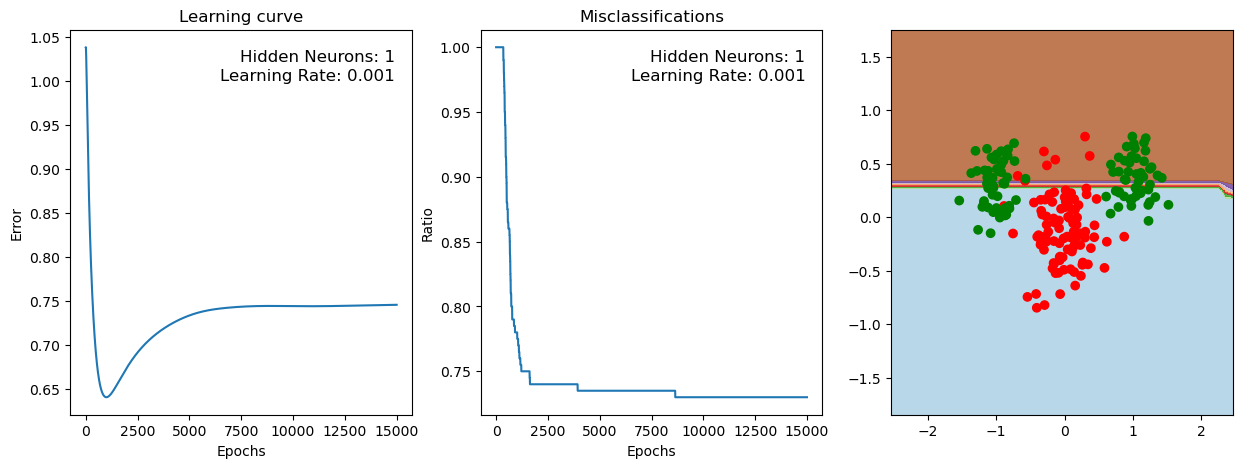
\includegraphics[width=10cm]{Labs/Lab 1/Lab 1b/Figure/1Hiddenlayer.png}
    \caption{Results of one hidden neuron}
    \label{fig:1Hidden}
\end{figure}

\begin{figure}[htb]
    \centering
    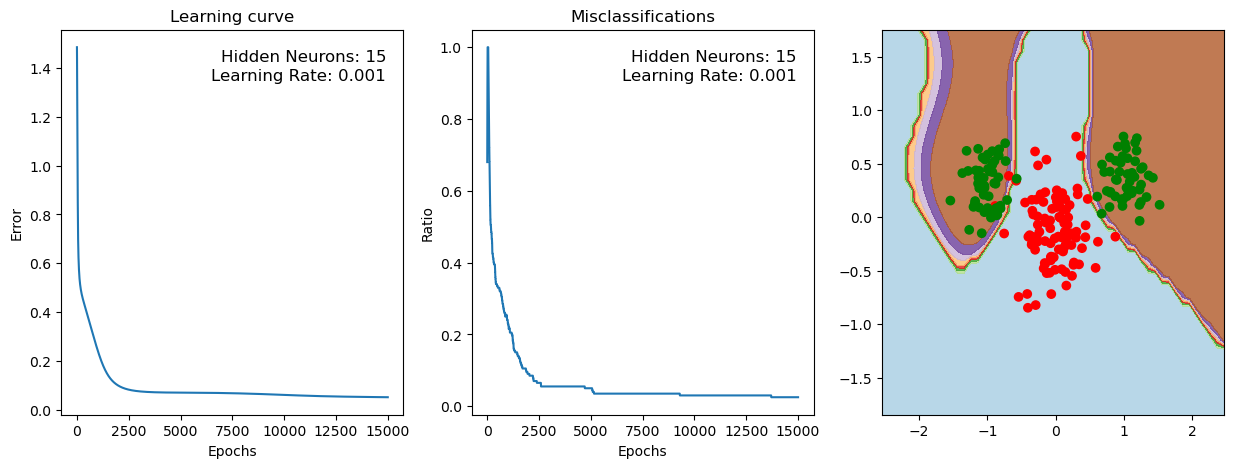
\includegraphics[width=10cm]{Labs/Lab 1/Lab 1b/Figure/15HiddenLayer.png}
    \caption{Results of 15 hidden neurons}
    \label{fig:15Hidden}
\end{figure}
\textbf{Generalization check:}
In this check we generated three scenarios. In the first one we subsample 25\% from each class randomly and train while the rest is for validation. In the second one we subsample 50\% for training and the rest for validation. In the third one we subsample 20\% from a subset of class A which is less than 1 and 80\% from a subset of a class where. class A is more than 0. \\
\\ What was discovered was that that was a overall low generalization error for scenario 1 and 2 if the hidden nodes were more than 1. A generalization error was noticed on most of the networks on scenario 3 however surprisingly they converged. The speed of their convergence had to do with how many hidden nodes there were. They were all trained with a learning rate of 0.0005 as and epochs of 15000 as these numbers allowed us to see the differences in their convergence more easier. Figure \ref{fig: 5 hidden 3 scenarios} is with 5 hidden neurons and Figure \ref{fig: 30 hidden 3 scenarios} is with 30 hidden neurons. The decision bound is drawn on the entire dataset. 
\begin{figure}[!htb]
    \centering
    \begin{subfigure}[b]{0.48\textwidth}
        \centering
        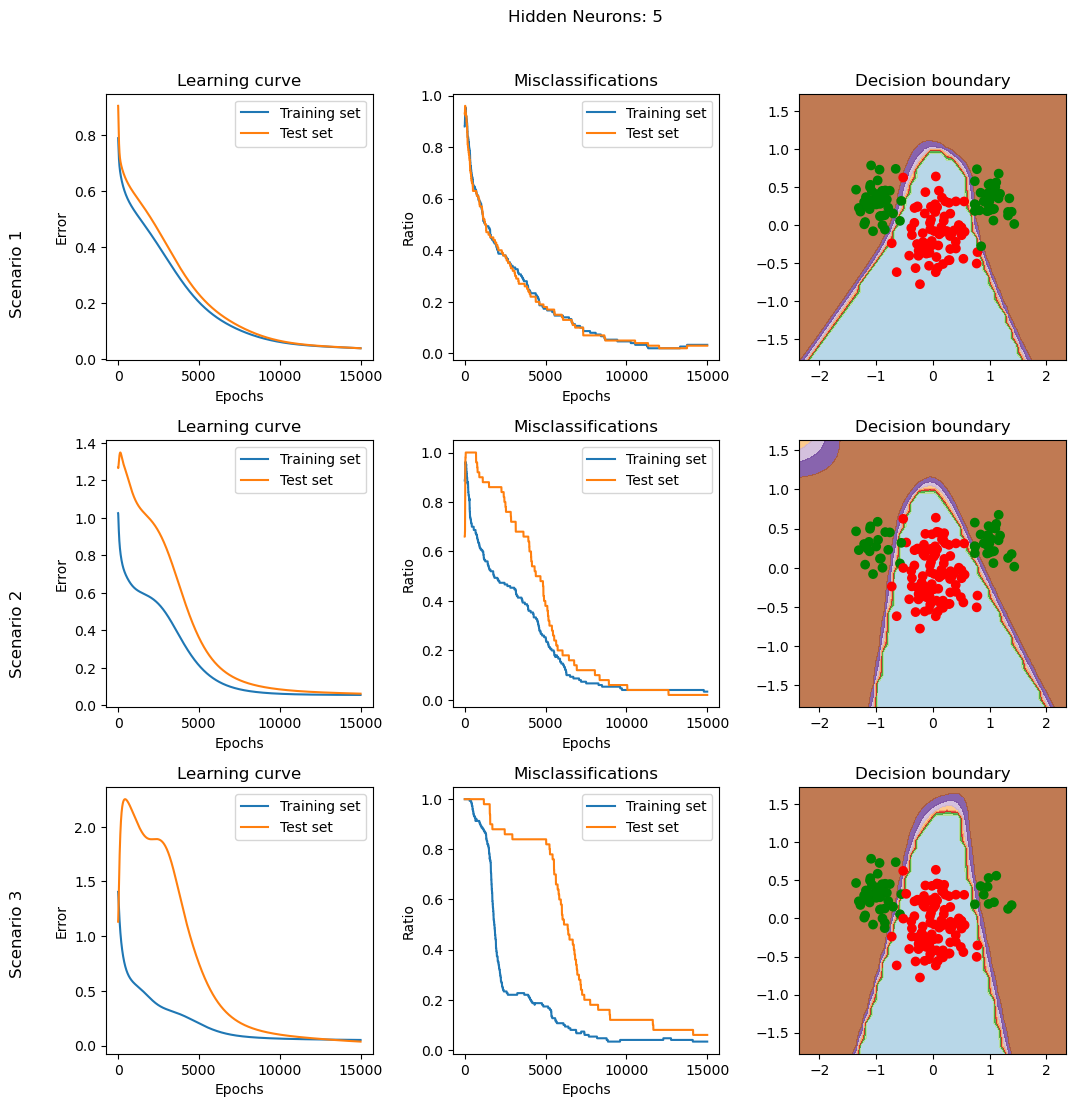
\includegraphics[width=\textwidth]{Labs/Lab 1/Lab 1b/Figure/3.1.1_5 hidden nodes.png}
        \caption{5 Hidden neurons for each scenario}
        \label{fig: 5 hidden 3 scenarios}
    \end{subfigure}%
    \hfill
    \begin{subfigure}[b]{0.48\textwidth}
        \centering
        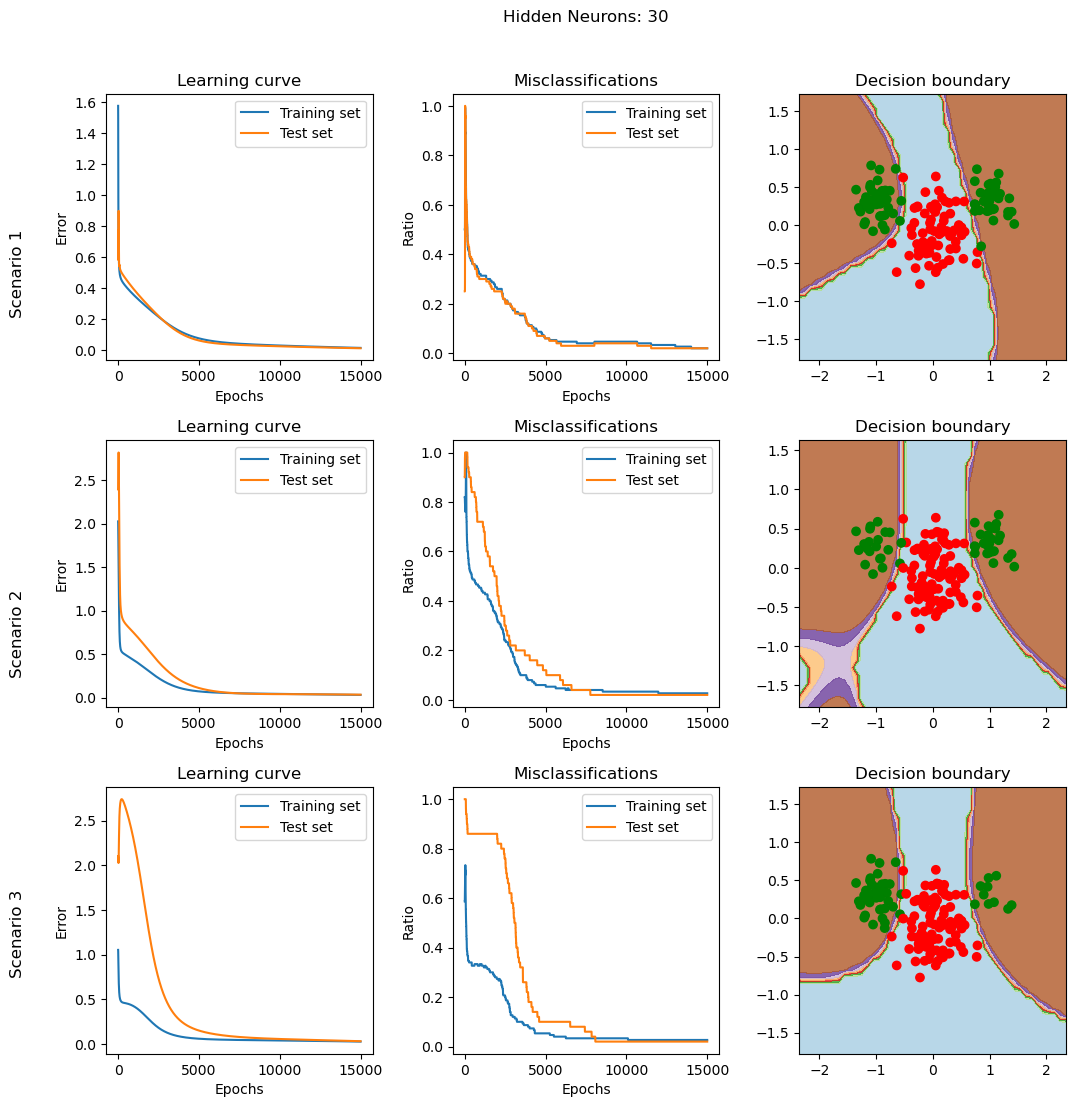
\includegraphics[width=\textwidth]{Labs/Lab 1/Lab 1b/Figure/3.1.1_30 hidden nodes.png}
        \caption{30 Hidden Neurons for each scenario}
        \label{fig: 30 hidden 3 scenarios}
    \end{subfigure}
    \caption{Comparative scenarios with different numbers of hidden neurons}
    \label{fig: comparative scenarios}
\end{figure}\\
\textbf{Regarding Sequential versus batch Learning}: We didn't notice much of a difference in terms in convergence other than sequential made "more changes" per epoch than batch learning. That figure has been purposefully omitted in order to stay within the 8 page limit.\\
\textbf{Function approximation of a Gaussian function:} In this part of the assignment we performed regression instead of classification. The purpose of the assignment was to see how well a multi layer perceptron can approximate a given function. The function we approximated was the well known bell shaped Gauss function:
$$
f(x, y) = e^{-(x^2+y^2)/10} - 0.5
$$
The bell function takes two variables as inputs and returns a number. The function can be plotted in three dimensional space where the x and y axis represent the inputs and the z-axis represents the output of the function. We plotted this with the plot\_surface function that is available in the python package matplotlib. The function can be seen in figure \ref{fig:gauss-function}

\begin{figure}[htbp]
    \centering
    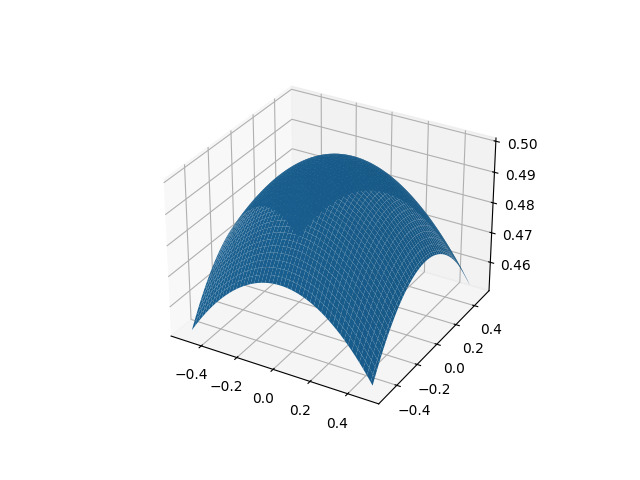
\includegraphics[width=0.5\textwidth]{Labs/Lab 1/Lab 1b/Figure/Figure_1.png}
    \caption{The bell shaped gauss function}
    \label{fig:gauss-function}
\end{figure}

We created a dataset by creating a mesh of x and y values in the interval -0.5 to 0.5. We used 80\% of the dataset as training data and then tested the model using the whole dataset. We varied the number of neurons in the hidden layer from 1-25 with a step size of 3, that is we used a model containing 1, 4, 7 all the way up to 25 neurons in the hidden layer. When training the network we used batch gradient descent with momentum and trained all of the networks for 10000 epochs. We used mean square error as the loss function. The mean square error for each of these models can be seen in table \ref{table:mse}:

\begin{table}
\begin{center}
    \begin{tabular}{|c|c|}
        \hline
         \# of hidden neurons & Mean square error \\
         \hline
         1 & 0.0001086\\
         \hline 
         4 & $5.96127*10^{-7}$\\
         \hline
         7 & $1.06032*10^{-5}$\\
         \hline
         10 & $2.01543*10^{-5}$\\
         \hline
         13 & $1.85068*10^{-6}$\\
         \hline
         16 & $1.78984*10^{-5}$\\
         \hline
         19 & $4.57150*10^{-5}$\\
         \hline
         22 & $1.49880*10^{-5}$\\
         \hline
         25 & $$\\
         \hline
    \end{tabular}
    \caption{Mean square errors as function of hidden neurons}
    \label{table:mse}
    \end{center}
\end{table}




\subsection{Multi-layer perceptron for time series prediction \textit{(ca.3 pages)}}

\textit{Here you do not have to introduce the problem or define Mackey-Glass time series, as you should focus on the results. You could divide them into two parts as the following two suggested subsections but you might as well keep your story under the main heading of this part of the assignment. Importantly, always clearly state what network architecture you use, crucially with the number of hidden nodes, systematically report average results with various manipulations (regularisation etc.) and pay attention to differences between training, validation and test errors. Illustrating the outcome of your network predictions along with the original chaotic time series can also be very helpful. Finally, since you compare two- and three-layer architectures, make sure that you do not jump to any conclusions based on a small number of simulations unless you have statistically convincing evidence (when you comare the mean performance measures, their second moment is also relevant). In this part it may be particularly desirable to rely on tables.}

\subsubsection{Three-layer perceptron for time series prediction - model selection, validation}

We created three subsets in this part of the assignment. The first one is the training subset, and the two others are validation and testing tests. The dataset consists of 1200 points: 800 for training, 200 for validation, and 200 for testing. The last 200 points were used in the end to measure how the best and the worst network design performance.

An illustration of how the data looks is an the figure below. 
\begin{figure}[htbp]
    \centering
    \includegraphics[width=0.5\textwidth]{Labs/Lab 1/Lab 1b/Part2/figure/}
    \caption{the data}
    \label{fig:gauss-function}
\end{figure}
We used TensorFlow, NumPy, and python Matplotlib to create the network. 

\subsubsection{Three-layer perceptron for noisy time series prediction with penalty regularisation}

\section{Final remarks \normalsize{\textit{(max 0.5 page)}}}
\textit{Please share your final reflections on the lab, its content and your own learning. Which parts of the lab assignment did you find confusing or not necessarily helping in understanding important concepts and which parts you have found interesting and relevant to your learning experience? \\
Here you can also formulate your opinion, interpretation or speculation about some of the simulation outcomes. Please add any follow-up questions that you might have regarding the lab tasks and the results you have produced.}

\end{document}
